%%=============================================================================
%% Resultaten
%%=============================================================================

\chapter{Resultaten}
\label{ch:resultaten}

Kijkend naar de resultaten van de tabeltransformatie van de dertig willekeurige documenten, die in appendix-deel \ref{ch:details-van-resultaten} bekeken kunnen worden, kan men enkele waarnemeingen maken. Zo ziet men dat \Gls{OCR} niet altijd nauwkeurig werkt, zeker niet wanneer de resolutie van de afbeelding laag is. Verder kan men, door de grafiek \ref{graph:resultaten} te bestuderen, merken dat de nauwkeurigheid van de tabeltransformatie afhankelijk is van de algoritme die gebruikt wordt voor tabelstructuuranalyse. 

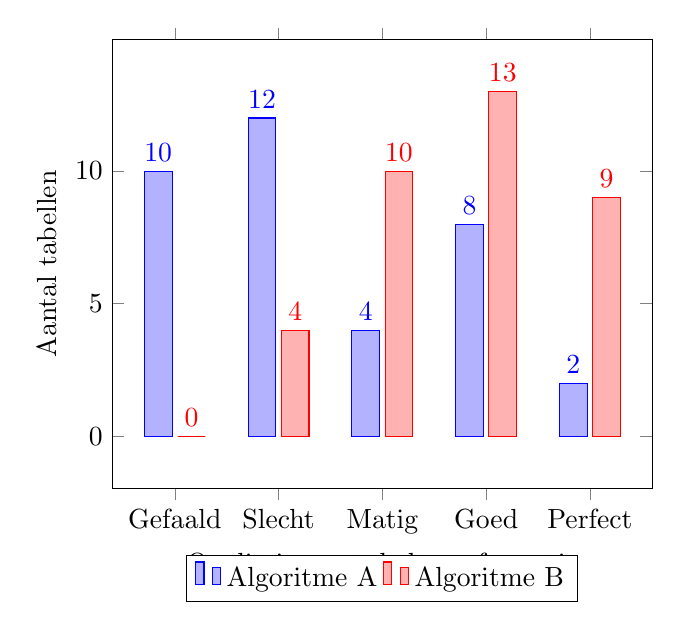
\begin{tikzpicture}
\begin{axis}[
    ybar,
    enlargelimits=0.15,
    legend style={at={(0.5,-0.15)},
      anchor=north,legend columns=-1},
    ylabel={Aantal tabellen},
    xlabel={Qualiteit van tabeltransformatie},
    symbolic x coords={Gefaald,Slecht,Matig,Goed,Perfect},
    xtick=data,
    nodes near coords,
    nodes near coords align={vertical},
    ]
    \addplot coordinates {(Gefaald,10) (Slecht,12) (Matig,4) (Goed,8) (Perfect,2)};
    \addplot coordinates {(Gefaald,0) (Slecht,4) (Matig,10) (Goed,13) (Perfect,9)};
    \legend{Algoritme A, Algoritme B}
\end{axis}
\label{graph:resultaten}
\end{tikzpicture}

Bij gebruik van de voorgestelde algoritme B is de slaagkans op een succesvolle tabeltransformatie merklijk groter dan bij gebruik van algoritme A. Verder kan men zien dat, hoewel een groot aantal goede en perfecte tabeltransformaties verkregen zijn, de hoeveelheid slechte en matige transformaties niet onbeduidend is.
